\chapter{Proposta}\label{cap:proposta}

Este trabalho apresenta um novo construtor para o \texttt{OpenMP} que facilita a implementação de algoritmos de aproximação. Assim como outros construtores da API, a proposta utiliza anotações de código, para identificar regiões que podem ser executadas de forma aproximada. A integração dessas anotações ao arcabouço do \texttt{OpenMP} assegura que as técnicas sejam portáteis e facilmente adaptáveis a diferentes trechos de código.

O \autoref{code:pragmaApprox} apresenta a anotação \texttt{pragma approx}, que delimita uma região de código a ser aproximada e especifica a técnica a ser aplicada. Múltiplas cláusulas podem ser combinadas em um único construtor para indicar diferentes parâmetros de aproximação. Entretanto, a implementação atual suporta apenas uma técnica de aproximação

\begin{sourcecode}[htb]\caption{\label{code:pragmaApprox}Sintaxe do construtor \texttt{approx}}
    \begin{lstlisting}[frame=single, language=C++]
        #pragma omp approx [clause, [[,]clause]]
    \end{lstlisting}
    \fonte{}
\end{sourcecode}

\section{Perforação de laço}\label{subsec:pragmaPerfo}

A cláusula \texttt{perfo} habilita o uso de perforação de laços (loop perforation), permitindo reduzir o número de iterações executadas. Essa cláusula deve ser utilizada em conjunto com a cláusula \texttt{for}, e suporta modificadores que definem tanto o algoritmo de perfuração quanto a taxa de descarte.
Os modificadores disponíveis são: \texttt{init}, \texttt{fini}, \texttt{small}, \texttt{large} e \texttt{default}.
A \autoref{code:pragmaPerfo} apresenta a sintaxe da cláusula.

\begin{sourcecode}[htb]
    \caption{\label{code:pragmaPerfo}Sintaxe da cláusula \texttt{perfo}}
    \begin{lstlisting}[frame=single, language=C++]
        #pragma omp approx perfo({init, fini, small, large, default}, \
                                 drop-rate)
    \end{lstlisting}
    \fonte{}
\end{sourcecode}

O modificador \texttt{init} descarta a quantidade especificada de iterações no início do laço.
Esse comportamento é implementado por meio de uma alteração na variável de indução, que ajusta o limite inferior do laço para cada \textit{thread}.
Dessa forma, quando a \textit{thread} assume sua fatia do laço, as primeiras iterações dessa fatia são descartadas. O comportamento dessa cláusula é apresentado na \autoref{fig:perfo_init}.

O modificador \texttt{fini} descarta as iterações finais do laço, de modo análogo ao \texttt{init}, afetando também os limites do laço por \textit{thread}. Seu comportamento é apresentado na \autoref{fig:perfo_fini}.

O modificador \texttt{small} aplica uma estratégia probabilística, na qual um valor aleatório é usado para decidir o descarte de iterações, com base em uma condição de módulo envolvendo a taxa de descarte.
Se a condição do valor aleatório ser igual à taxa for satisfeita, a variável de indução é incrementada pela taxa de descarte, efetivamente pulando algumas iterações, como mostra a \autoref{fig:perfo_small}.

A \autoref{eq:perfo}, apresenta a fórmula usada para verifica a condição. As variáveis envolvidas nessa fórmula são:

\begin{itemize}
    \item $\xi$: Número aleatório.
    \item $ub$: Limite superior do laço.
    \item $lb$: Limite inferior do laço.
    \item $d$: Taxa de descarte.
\end{itemize}

\begin{equation}
    \label{eq:perfo}
    \xi mod ((ub - lb) + ub) mod d
\end{equation}

O modificador \texttt{large} aplica uma perfuração mais agressiva, incrementando diretamente a variável de indução pela taxa de descarte.
Essa substituição é feita em tempo de execução, interceptando a lógica padrão de incremento ou decremento e substituindo-a por uma chamada de função que ajusta a variável de indução conforme a taxa. A \autoref{fig:perfo_large} o seu comportamento no laço.

O modificador \texttt{default} apresenta comportamento semelhante ao \texttt{large}, porém a taxa de descarte é aplicada em tempo de compilação, eliminando a sobrecarga associada a chamadas adicionais durante a execução.

\begin{figure}[htb]
    \centering

    \begin{minipage}[b]{0.80\textwidth}
        \centering
        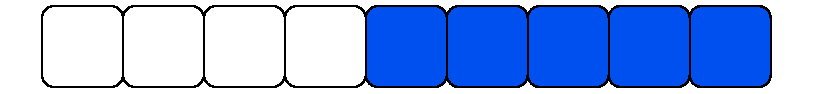
\includegraphics[width=\textwidth]{figuras/perfo_init.pdf}
        \caption{Comportamento do modificador \texttt{init}.}
        \label{fig:perfo_init}
    \end{minipage}
    \hfill

    \begin{minipage}[b]{0.80\textwidth}
        \centering
        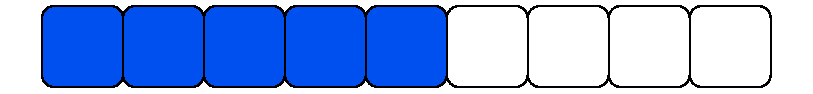
\includegraphics[width=\textwidth]{figuras/perfo_fini.pdf}
        \caption{Comportamento do modificador \texttt{fini}.}
        \label{fig:perfo_fini}
    \end{minipage}

    \begin{minipage}[b]{0.80\textwidth}
        \centering
        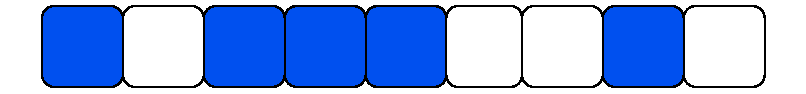
\includegraphics[width=\textwidth]{figuras/perfo_small.pdf}
        \caption{Comportamento do modificador \texttt{small}.}
        \label{fig:perfo_small}
    \end{minipage}

    \begin{minipage}[b]{0.80\textwidth}
        \centering
        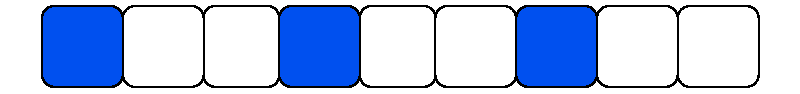
\includegraphics[width=\textwidth]{figuras/perfo_large.pdf}
        \caption{Comportamento do modificador \texttt{large}.}
        \label{fig:perfo_large}
    \end{minipage}

    \caption{Característica de cada modificador do \texttt{large}.}
    \label{fig:exemploMinipage}
\end{figure}

\section{Aproximação de ponto flutuante}\label{subsec:pragmaFastmath}

A cláusula \texttt{fastmath} habilita otimizações de ponto flutuante, seguindo a semântica do parâmetro de compilação \texttt{--fast-math} do compilador \texttt{Clang}~\cite{clangffast}. Quando aplicada, o compilador extrai a região de código anotada e adiciona metadados indicando que essa região permite otimizações agressivas de ponto flutuante.

A principal diferença entre os dois métodos está no fato de que a cláusula \texttt{fastmath} oferece controle mais granular, permitindo que as otimizações sejam aplicadas apenas na região especificada. Em contraste, o parâmetro global \texttt{--fast-math} força a aplicação dessas otimizações em todo o módulo de compilação. A \autoref{code:pragmaFastmath} apresenta a sintaxe da cláusula.

\begin{sourcecode}[htb]\caption{\label{code:pragmaFastmath}Sintaxe da cláusula \texttt{fastmath}}
    \begin{lstlisting}[frame=single, language=C++]
        #pragma omp approx fastmath
    \end{lstlisting}
    \fonte{}
\end{sourcecode}
Uma característica fundamental dessa cláusula está nas otimizações relacionadas à associatividade das operações de ponto flutuante. Isso permite que o compilador reordene operações de modo a melhorar o desempenho. Embora a reordenação seja válida para números reais, na aritmética de ponto flutuante ela pode produzir resultados numericamente distintos devido aos erros de arredondamento acumulados em cada operação. Esse comportamento é ilustrado na \autoref{fig:floatPoint}.

A \autoref{code:exFastmath} apresenta um exemplo prático do uso da cláusula. A função \textit{sqrt}, por exemplo, normalmente requer verificações adicionais para lidar com entradas inválidas, como valores negativos ou \textit{NaN} (\textit{Not a Number}). Ao aplicar \texttt{fastmath}, o compilador assume que essas entradas não ocorrerão, emitindo diretamente a instrução de hardware \textit{sqrt}, sem checagens extras, o que reduz a sobrecarga e melhora o desempenho.

\begin{sourcecode}[htb]\caption{\label{code:exFastmath}Sintaxe da clausula \texttt{fastmath}}
    \begin{lstlisting}[frame=single, language=C++]
        float sqrt_approx(float x)
        {
            #pragma omp approx fastmath
            {
                return sqrt(x);
            }
        }
    \end{lstlisting}
    \fonte{}
\end{sourcecode}

\section{Descarte de Tarefas}\label{subsec:pragmaTaskdrop}

O conceito de tarefas no \texttt{OpenMP} permite a execução assíncrona de regiões de código. Quando uma \textit{thread} encontra uma região anotada com a cláusula \texttt{task}, um objeto de tarefa é criado para ser executado posteriormente. Essa tarefa é então escalonada dinamicamente, podendo ser executada por qualquer outra \textit{thread}. Esse modelo de execução é particularmente útil em computações heterogêneas e irregulares, pois permite uma distribuição dinâmica da carga de trabalho entre as \textit{threads}~\cite{ayguade2007,openmpapi52}.

O construtor \texttt{taskloop} estende esse conceito para laços. Cada laço é particionado em pedaços, definidos pelo parâmetro \texttt{grainsize}, e uma tarefa é criada para cada pedaço. Essas tarefas podem então ser executadas de forma independente por diferentes \textit{threads}.

\begin{figure}[htb]
    \centering
    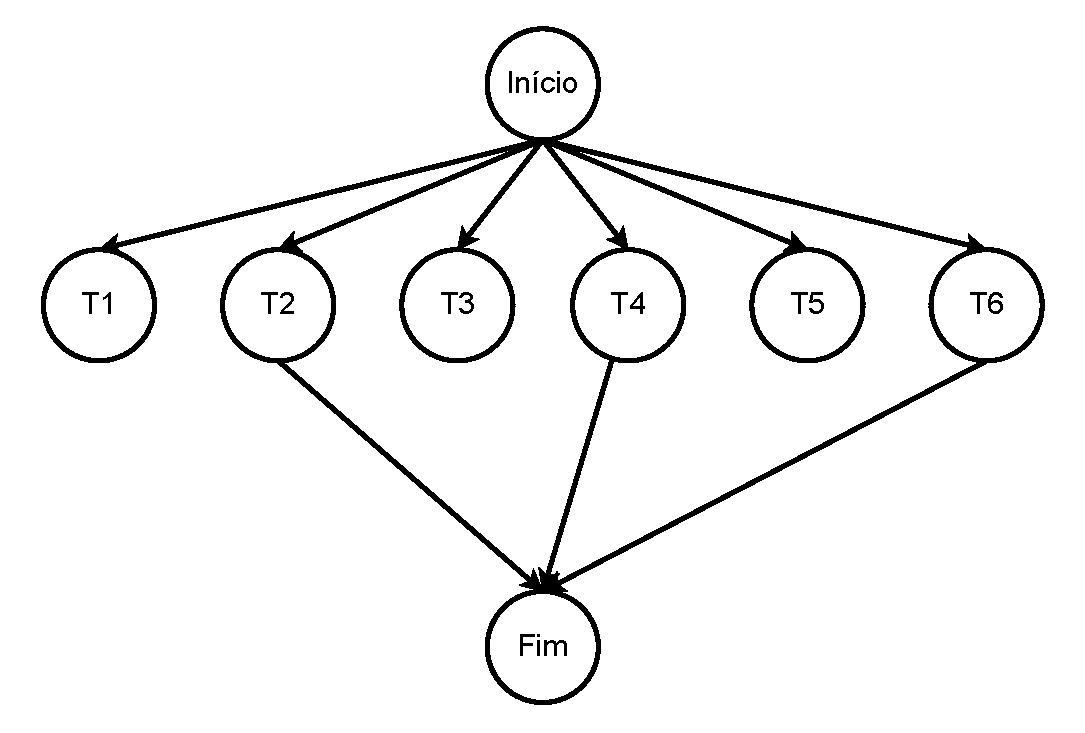
\includegraphics[width=\textwidth]{figuras/task.pdf}
    \caption{Modelo de execução da cláusula \texttt{drop}.}
    \label{fig:task_drop}
\end{figure}

Neste trabalho, propomos a cláusula \texttt{drop}, que pode ser usada em conjunto com \texttt{taskloop} para implementar uma estratégia de aproximação baseada no descarte de tarefas. De forma similar à técnica de perforação de laço, essa cláusula permite que o usuário especifique uma taxa de descarte, que define quantas tarefas serão eliminadas. A \autoref{eq:perfo} é utilizada para determinar quais tarefas devem ser descartadas.

A \autoref{fig:task_drop} ilustra esse processo, e o \autoref{code:pragmaDrop} apresenta a sintaxe da cláusula.

\begin{sourcecode}[htb]
    \caption{\label{code:pragmaDrop}Sintaxe da cláusula \texttt{drop}}
    \begin{lstlisting}[frame=single, language=C++]
        #pragma omp approx taskloop drop(drop-rate)
    \end{lstlisting}
    \fonte{}
\end{sourcecode}

O \autoref{code:exDrop} mostra um exemplo de uso da cláusula \texttt{drop} em conjunto com \texttt{taskloop} para aproximar o resultado de uma soma:

\begin{sourcecode}[htb]
    \caption{\label{code:exDrop}Exemplo de uso da cláusula \texttt{drop}}
    \begin{lstlisting}[frame=single, language=C++]
    #pragma omp parallel
    {
        #pragma omp single
        {
            #pragma omp approx taskloop drop(3) reduction(+ : sum)
            {
                for (int i = 0; i < N; i++) {
                    sum += values[i];
                }
            }
        }
    }
    \end{lstlisting}
    \fonte{}
\end{sourcecode}

\section{Memoização}\label{subsec:pragmaMemo}

A cláusula \texttt{memo} habilita otimizações de memoização, permitindo o reuso de resultados previamente calculados. Essa estratégia é particularmente útil para funções em que a relação entre entrada e saída se mantém estável ao longo do tempo, desde que a execução da mesma região de código produza resultados consistentes, independentemente das entradas específicas.

O \autoref{code:pragmaMemo} apresenta a sintaxe da cláusula \texttt{memo}. Essa cláusula deve ser utilizada em conjunto com a diretiva \texttt{shared} para garantir que, em tempo de execução, as variáveis indicadas possam ser acessadas. Opcionalmente, o modificador \texttt{threshold} pode ser especificado para definir um limite aceitável de erro entre os resultados que serão reutilizados.

\begin{sourcecode}[htb]
    \caption{\label{code:pragmaMemo}Sintaxe da cláusula \texttt{memo}}
    \begin{lstlisting}[frame=single, language=C++]
        #pragma omp approx memo shared([variables]) [threshold(error-limit)]
    \end{lstlisting}
    \fonte{}
\end{sourcecode}

\begin{figure}[htb]
    \centering
    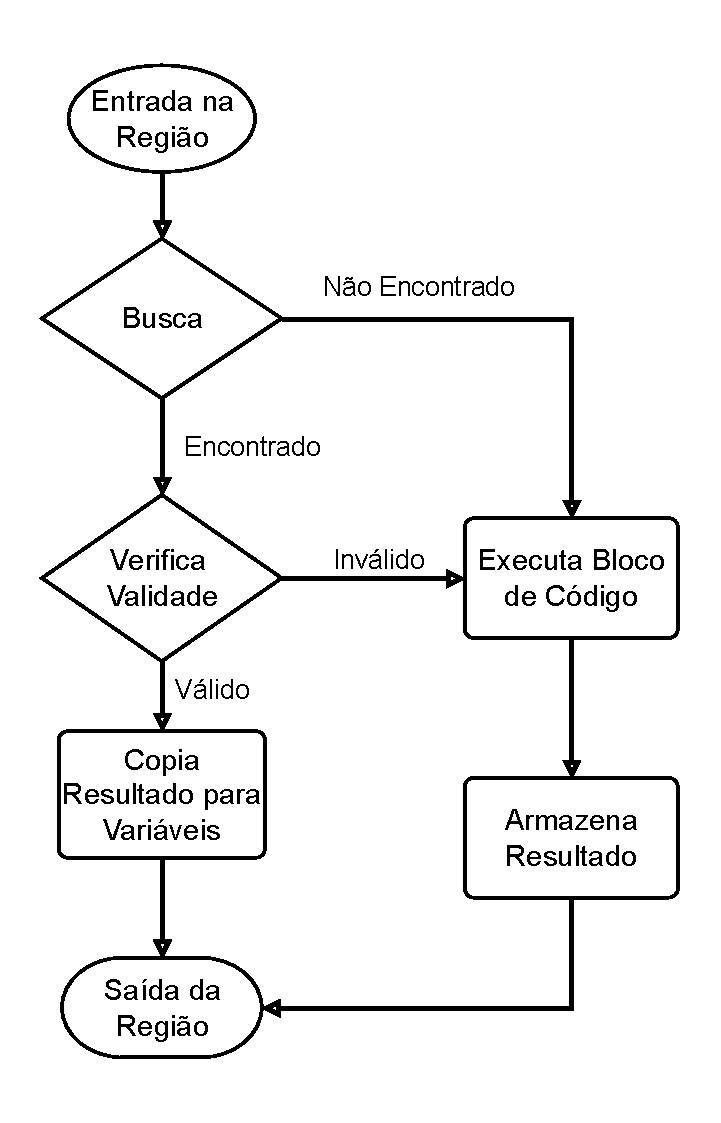
\includegraphics[scale=0.5]{figuras/memo.pdf}
    \caption{Modelo de execução da cláusula \texttt{memo}.}
    \label{fig:memo}
\end{figure}

Internamente, a técnica é implementada usando uma árvore AVL, cujos nós folha são estruturas \textit{hash map}. Em tempo de execução, as chamadas à função interceptam a região de código anotada e verificam se existe algum resultado previamente armazenado válido para aquela região. Se houver um resultado válido, ele é reutilizado; caso contrário, o bloco de código é executado normalmente e o resultado é armazenado para uso futuro. O fluxo de execução está ilustrado na \autoref{fig:memo}. É importante ressaltar que, nesta versão da implementação, a verificação de validade é feita exclusivamente com base na região de código, sem considerar diretamente os valores de entrada. Portanto, o reuso é determinado apenas pela execução da mesma região, independentemente das entradas fornecidas.

Quando o usuário especifica um limiar através do modificador \texttt{threshold}, a execução passa a incluir uma verificação que mede a diferença relativa entre os resultados da região. Se essa diferença estiver dentro do limite definido, o valor é armazenado e considerado válido para reuso. Caso nenhum limiar seja especificado, os valores previamente calculados são sempre reutilizados, sem verificação adicional. O \autoref{code:exMemo} apresenta um exemplo de uso da cláusula \texttt{memo} aplicado a um laço, usando um limiar de 10\%. Com a memoização habilitada, execuções repetidas dessa região de código podem ser substituídas por valores previamente calculados, respeitando o limite de erro definido.

\begin{sourcecode}[htb]
    \caption{\label{code:exMemo}Exemplo de uso da cláusula \texttt{memo}}
    \begin{lstlisting}[frame=single, language=C++]
        #pragma omp approx memo shared(sum) threshold(0.1)
        {
            for (int i = 0; i < N; i++) {
                sum += values[i];
            }
        }
    \end{lstlisting}
    \fonte{}
\end{sourcecode}
